\documentclass[journal]{IEEEtran}
\usepackage[a5paper, margin=10mm]{geometry}
%\usepackage{lmodern} % Ensure lmodern is loaded for pdflatex
\usepackage{tfrupee} % Include tfrupee package


\setlength{\headheight}{1cm} % Set the height of the header box
\setlength{\headsep}{0mm}     % Set the distance between the header box and the top of the text


%\usepackage[a5paper, top=10mm, bottom=10mm, left=10mm, right=10mm]{geometry}

%
\setlength{\intextsep}{10pt} % Space between text and floats

\makeindex


\usepackage{cite}
\usepackage{amsmath,amssymb,amsfonts,amsthm}
\usepackage{algorithmic}
\usepackage{graphicx}
\usepackage{textcomp}
\usepackage{xcolor}
\usepackage{txfonts}
\usepackage{listings}
\usepackage{enumitem}
\usepackage{mathtools}
\usepackage{gensymb}
\usepackage{comment}
\usepackage[breaklinks=true]{hyperref}
\usepackage{tkz-euclide} 
\usepackage{listings}
\usepackage{multicol}
\usepackage{xparse}
\usepackage{gvv}
%\def\inputGnumericTable{}                                 
\usepackage[latin1]{inputenc}                                
\usepackage{color}                                            
\usepackage{array}                                            
\usepackage{longtable}                                       
\usepackage{calc}                                             
\usepackage{multirow}                                         
\usepackage{hhline}                                           
\usepackage{ifthen}                                               
\usepackage{lscape}
\usepackage{tabularx}
\usepackage{array}
\usepackage{float}
\usepackage{ar}
\usepackage[version=4]{mhchem}


\newtheorem{theorem}{Theorem}[section]
\newtheorem{problem}{Problem}
\newtheorem{proposition}{Proposition}[section]
\newtheorem{lemma}{Lemma}[section]
\newtheorem{corollary}[theorem]{Corollary}
\newtheorem{example}{Example}[section]
\newtheorem{definition}[problem]{Definition}
\newcommand{\BEQA}{\begin{eqnarray}}
\newcommand{\EEQA}{\end{eqnarray}}

\theoremstyle{remark}


\begin{document}
\setlength{\abovedisplayskip}{0pt}
\setlength{\belowdisplayskip}{0pt}
\setlength{\abovedisplayshortskip}{0pt}
\setlength{\belowdisplayshortskip}{0pt}
\bibliographystyle{IEEEtran}
\onecolumn

\title{2.8.10}
\author{Jnanesh Sathisha Karmar- EE25BTECH11029}
\maketitle


\renewcommand{\thefigure}{\theenumi}
\renewcommand{\thetable}{\theenumi}
\textbf{Question} If with reference to the right handed system of mutually perpendicular unit vectors
$\hat{i},\hat{j}$ and $\hat{k}, \vec{\alpha} = 3\hat{i}-\hat{j},\vec{\beta} = 2\hat{i} +\hat{j} - 3\hat{k},$ then express $\beta$ in the form $\beta =\beta_1 +\beta_2$ where $\beta_1$ is parallel to $\alpha$ and $\beta_2$ is perpendicular to $\alpha$ .

\textbf{Solution}
Given details:
\begin{align}
    \vec{\alpha} &= 3\hat{i}-\hat{j}=\myvec{3 \\ -1\\0}\\\vec{\beta} &= 2\hat{i} +\hat{j} - 3\hat{k}=\myvec{2\\1\\-3}
\end{align}

$\beta_1$ is a projection of $\beta$ on $\alpha$\\
The projection formula for projection is: 
\begin{align}
\beta_1&=\frac{\vec{\beta^T}\vec{\alpha}}{\norm{\vec{\alpha^2}}}\vec{\alpha}\\
&=\frac{\myvec{2&&1&&-3}\myvec{3\\-1\\0}}{\brak{3}^2+\brak{-1}^2+\brak{0}^2}\myvec{3\\-1\\0}\\
&=\frac{5}{10}\myvec{3\\-1\\0}\\
&=\myvec{\frac{3}{2}\\ \frac{-1}{2}\\ 0}
\end{align}
Now according to the given equation :
\begin{align}
    \beta&=\beta_1+\beta_2\\
    \beta_2&=\beta-\beta_1\\
    \beta_2&=\myvec{2\\1\\-3}-\myvec{\frac{3}{2}\\ \frac{-1}{2}\\0}\\
    \beta_2&=\myvec{\frac{1}{2}\\ \frac{3}{2}\\-3}
\end{align}
Lets verify wheter $\beta_2$ is perpendicular to $\alpha$\\
For that:
\begin{align}
    \alpha^T.\beta_2&=0\\
    \myvec{3&&-1&&0}\myvec{\frac{1}{2}\\ \frac{3}{2}\\-3}&=\myvec{0}
\end{align}
Therefore $\beta_2$ is perpendicular to $\alpha$

Therefore $\beta$ is:
\begin{align}
    \beta&=\beta_1+\beta_2\\
    \beta&=\myvec{\frac{3}{2}\\ \frac{-1}{2}\\0}+\myvec{\frac{1}{2}\\ \frac{3}{2}\\-3}
\end{align}
Performing QR decomposition on the matrix $\myvec{\alpha&&\beta}$
\begin{align}
    \vec{A}=\myvec{\alpha &&\beta}=\myvec{3&& 2\\-1 && 1 \\ 0 && -3}
\end{align}
Finding $\vec{q_1}\brak{\text{normalized}\  \alpha}$
\begin{align}
    \norm{\alpha}&=\sqrt{\myvec{\alpha}\myvec{\alpha}^T}=\sqrt{9+1}=\sqrt{10}\\
    \vec{q_1}&=\frac{\vec{\alpha}}{\norm{\vec{\alpha}}}=\myvec{\frac{3}{\sqrt{10}}&&\frac{-1}{\sqrt{10}}&&0}
\end{align}
The projection of $\beta$ on $\vec{q_1}$\\
projection coefficient:
\begin{align}
    \vec{r_{12}}=\vec{q_1^T}\vec{\beta}=\frac{3}{\sqrt{10}}.2+\frac{-1}{\sqrt{10}}+0=\frac{5}{\sqrt{10}}
\end{align}
projection:
\begin{align}
    proj\brak{\vec{\beta}}_{q_1}=\vec{r_{12}}.\vec{q_1}=\frac{5}{\sqrt{10}}.\myvec{\frac{3}{\sqrt{10}}&&\frac{-1}{\sqrt{10}}&&0}=\myvec{1.5 && -0.5 &&-3}
\end{align}
subtract projection from $\beta$:
\begin{align}
    \vec{u_1}=\beta-proj\brak{\vec{\beta}}_{q_1}=\myvec{0.5&&1.5&&&&-3}
\end{align}
we normalize $\vec{u_2}$ to get $\vec{q_2}$\\
compute $\norm{\vec{u_2}}$
\begin{align}
    \norm{u_2}&=\sqrt{\myvec{u_2}\myvec{u_2}^T}=\sqrt{11.5}\\
    \vec{q_2}&=\frac{\vec{u_2}}{\norm{u_2}}=\myvec{\frac{0.5}{\sqrt{11.5}}&& \frac{1.5}{\sqrt{11.5}}&&\frac{-3}{\sqrt{11.5}}}
\end{align}
$\vec{Q}$'s columns are $\vec{q_1}$ and $\vec{q_2}$
\begin{align}
    \vec{Q}=\myvec{3 && 0.5 \\ -1 && 1.5 \\ 0 && -3}
\end{align}
$\vec{R}$ is:
\begin{align}
    \vec{R}=\myvec{\sqrt{10} && \frac{5}{\sqrt{10}}\\0 &&\sqrt{11.5}}
\end{align}
\newpage
\begin{figure}[H]
    \centering
    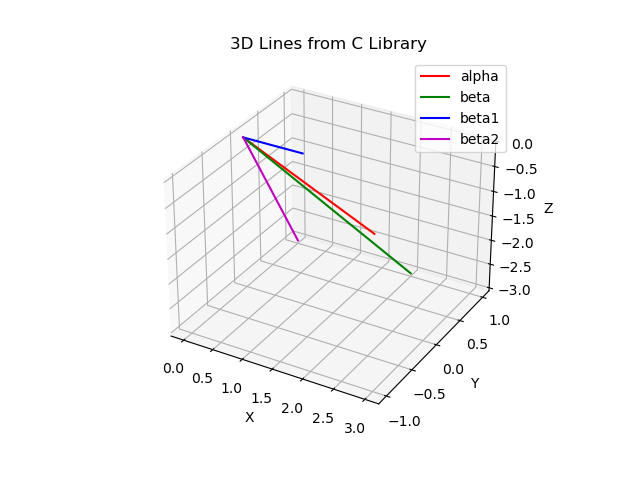
\includegraphics[width=0.9\columnwidth]{figs/fig2.png}
    \caption{vectors}
    \label{fig:placeholder_1}
\end{figure}
\end{document}